\documentclass[10pt, a5paper]{report}

\usepackage[T1]{fontenc}%
\usepackage[utf8]{inputenc}% encodage utf8
\usepackage[francais]{babel}% texte fran�ais
\usepackage[final]{pdfpages}
\usepackage{modules-livret}% style du livret
\usepackage{url}
%\usepackage{init-preambule}
\pagestyle{empty}

% % % % % % % % % % % % % % % % % % % % % % % % % % % % % % % % % % % % % % % % % % % % % % % % % % % % % % % 
\begin{document}

%---------------------- % % % Personnalisation des couleurs % % % ----------- MOUTARDE --------
\definecolor{couleurFonce}{RGB}{170,110,0} % Couleur du Code APOGEE
\definecolor{couleurClaire}{RGB}{222,190,137} % Couleur du fond de la bande
\definecolor{couleurTexte}{RGB}{255,255,255} % Couleur du texte de la bande
%------------------------------------------------------------------------------------------



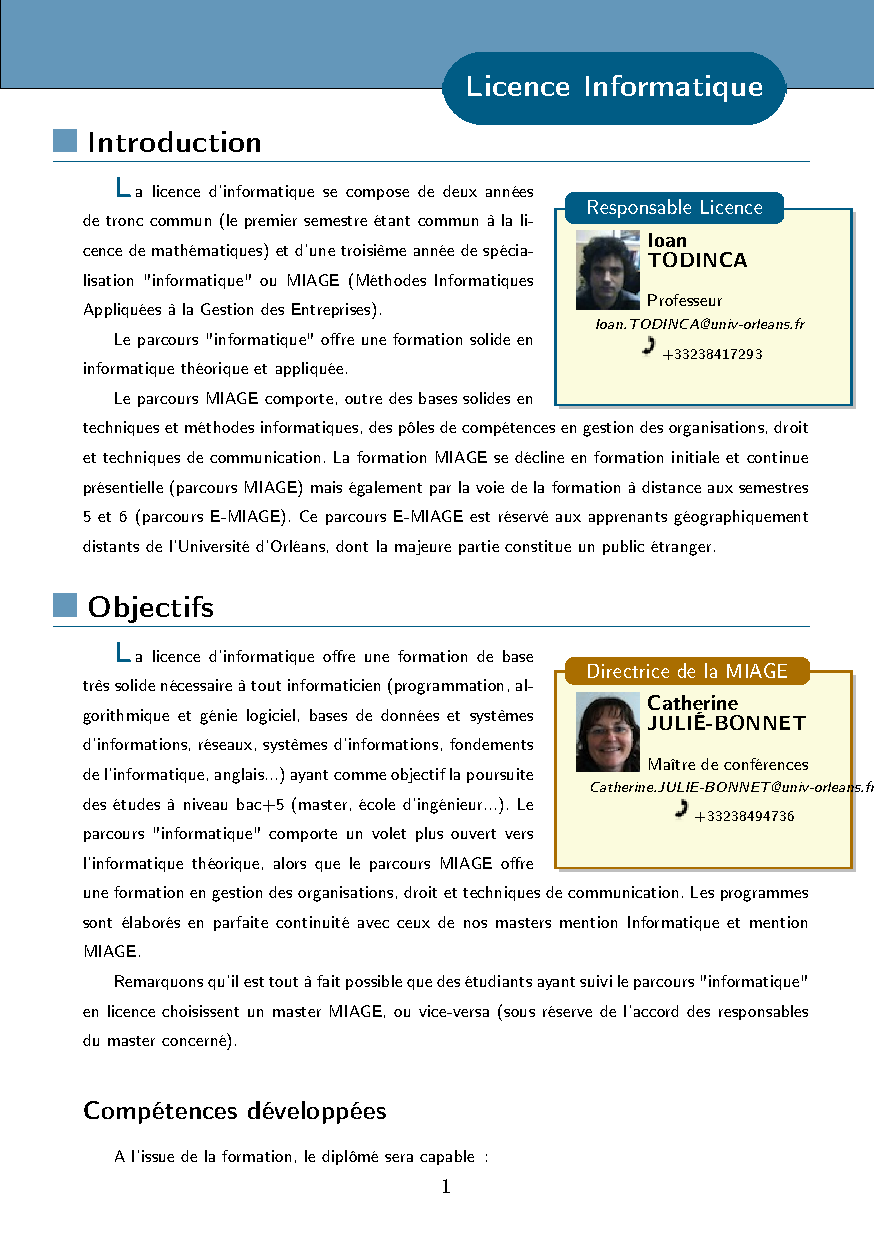
\includepdf[fitpaper,pages=-]{Preambule_Info_MasterMIAGE_S1S2.pdf}

%==========================================================================================
\module[codeApogee={UE11}, 
titre={Analyse de données}, 
COURS={18}, 
TD={}, 
TP={24}, 
CTD={}, 
TOTAL={42}, 
SEMESTRE={Semestre 1}, 
COEFF={3}, 
ECTS={3}, 
MethodeEval={Contrôle continue et terminal}, 
ModalitesCCSemestreUn={CC et CT}, 
ModalitesCCSemestreDeux={CT}, 
%CalculNFSessionUne={$\frac{(CC+2*CT)}{3}$}, 
%CalculNFSessionDeux={CT}, 
NoteEliminatoire={7}, 
nomPremierResp={Didier CHEVEAU}, 
emailPremierResp={Didier.CHEVEAU@univ-orleans.fr}, 
nomSecondResp={}, 
emailSecondResp={}, 
langue={Français}, 
nbPrerequis={1}, 
descriptionCourte={true}, 
descriptionLongue={true}, 
objectifs={true}, 
ressources={true}, 
bibliographie={false}] 
{
Unité obligatoire. 
} 
{
Principales méthodes d'analyse de données:
\begin{itemize} 
\item Statistiques descriptives usuelles (rappels)
\item Analyse en Composantes Principales (ACP)
\item Analyse Factorielle des Correspondances (AFC)
\item Analyse des Correspondances Multiples (ACM)
\item Méthodes de Classification (hiérarchique et non hiérarchique)
\end{itemize} 
Travaux Dirigés:
\begin{itemize} 
\item Apprentissage de SAS
\item Recueil, nettoyage, recodage, mise en forme des données
\item Applications des méthodes vues en cours à des jeux de données exemples.
\end{itemize} 
} 
{Notions d'algèbre linéaire.} 
{\begin{itemize} 
  \ObjItem Savoir analyser et synthétiser un jeu de données par des techniques
statistiques descriptives ou multivariées usuelles.
  \ObjItem Savoir manipuler les
procédures d'analyse statistique du logiciel SAS.
\end{itemize} 
} 
{Ressources} 
{Biblio} 
 
\vfill

%==========================================================================================
\module[codeApogee={UE 12}, 
titre={Types abstraits de données}, 
COURS={18}, 
TD={24}, 
TP={}, 
CTD={}, 
TOTAL={42}, 
SEMESTRE={Semestre 1}, 
COEFF={4}, 
ECTS={4}, 
MethodeEval={Contrôle continue et terminal}, 
ModalitesCCSemestreUn={CC et CT}, 
ModalitesCCSemestreDeux={CT}, 
%CalculNFSessionUne={$\frac{(CC+2*CT)}{3}$}, 
%CalculNFSessionDeux={CT}, 
NoteEliminatoire={7}, 
nomPremierResp={Jean-Jacques LACRAMPE}, 
emailPremierResp={Jean-Jacques.LACRAMPE@univ-orleans.fr}, 
nomSecondResp={}, 
emailSecondResp={}, 
langue={Français}, 
nbPrerequis={1}, 
descriptionCourte={true}, 
descriptionLongue={true}, 
objectifs={true}, 
ressources={true}, 
bibliographie={false}] 
{
Unité obligatoire. 
} 
{
\begin{itemize} 
\item Génie logiciel :
distinction spécification/implémentation,
indépendance de l'application par rapport à l'implémentation,
multiplicité des implémentations, raffinements successifs,
modularité, réutilisabilité.
\item Présentation d'un formalisme pour les spécifications de types abstraits
algébriques :
profils, préconditions, axiomes,
propriétés : spécifications suffisantes, spécifications complètes.
notion de modèle; le cas particulier du modèle des termes de la sigmaalgèbre.
\item Mise en oeuvre en Ada :
types abstraits, fonctions de classe,
implémentations génériques, classe des implémentations,
sigma-modèle, optimisation du modèle.
\item Catalogue de structures : piles, files, liste, tables, arbres ...
\end{itemize} 
} 
{Pratique des structures de données, notion de règle de réécriture, algèbres
de termes.Connaissance d'Ada 2005 (généricité, programmation par classe).} 
{\begin{itemize} 
  \ObjItem Développer les capacités d'abstraction et de généralisation et connaître les
raisonnements par récurrence et induction.
\end{itemize} 
} 
{Ressources} 
{Biblio} 
 
\vfill

%==========================================================================================
\module[codeApogee={UE 13}, 
titre={Complexité des algorithmes}, 
COURS={18}, 
TD={18}, 
TP={}, 
CTD={}, 
TOTAL={36}, 
SEMESTRE={Semestre 1}, 
COEFF={3}, 
ECTS={3}, 
MethodeEval={Contrôle continue et terminal}, 
ModalitesCCSemestreUn={CC et CT}, 
ModalitesCCSemestreDeux={CT}, 
%CalculNFSessionUne={$\frac{(CC+2*CT)}{3}$}, 
%CalculNFSessionDeux={CT}, 
NoteEliminatoire={7}, 
nomPremierResp={Jérôme DURAND-LOSE}, 
emailPremierResp={Jerome.DURAND-LOSE@univ-orleans.fr}, 
nomSecondResp={}, 
emailSecondResp={}, 
langue={Français}, 
nbPrerequis={1}, 
descriptionCourte={true}, 
descriptionLongue={true}, 
objectifs={true}, 
ressources={true}, 
bibliographie={false}] 
{
Unité obligatoire. 
} 
{
\begin{itemize} 
\item Notions de complexité.
\item Coût en temps et en espace, dans le pire des cas et en moyenne.
\item Problèmes d'optimalité.
\item Mesure empirique, test de performance.
\item Coût du passage à l'échelle.
\item Calcul formel de la complexité (et temps) : itératif et récursif.
\item De nombreux exemples illustrent le cours, parmi lesquels on peut citer :
  \begin{itemize} 
  \item algorithmes de recherche, algorithmes de tri (Quick-sort, Heap-sort, tri radix...),
  \item algorithmes sur les graphes (composantes connexes, chemin minimal...).
  \end{itemize} 
\end{itemize} 
} 
{Algorithmique et programmation.} 
{\begin{itemize} 
  \ObjItem Être capable de prédire si un algorithme devrait ou non aboutir à un
programme ayant un temps de calcul / un besoin en espace raisonnable.
  \ObjItem Être capable d'estimer les ressources nécessaires quand le volume de
données à traiter augmente.
\end{itemize} 
} 
{Ressources} 
{Biblio} 
 
\vfill

%==========================================================================================
\module[codeApogee={UE 14}, 
titre={Langages formels et automates}, 
COURS={18}, 
TD={24}, 
TP={}, 
CTD={}, 
TOTAL={42}, 
SEMESTRE={Semestre 1}, 
COEFF={3}, 
ECTS={3}, 
MethodeEval={Contrôle continue et terminal}, 
ModalitesCCSemestreUn={CC et CT}, 
ModalitesCCSemestreDeux={CT}, 
%CalculNFSessionUne={$\frac{(CC+2*CT)}{3}$}, 
%CalculNFSessionDeux={CT}, 
NoteEliminatoire={7}, 
nomPremierResp={Wadoud BOUSDIRA}, 
emailPremierResp={Wadoud.BOUSDIRA@univ-orleans.fr}, 
nomSecondResp={}, 
emailSecondResp={}, 
langue={Français}, 
nbPrerequis={1}, 
descriptionCourte={true}, 
descriptionLongue={true}, 
objectifs={true}, 
ressources={true}, 
bibliographie={false}] 
{
Unité obligatoire. 
} 
{
\begin{itemize} 
\item Généralités
  \begin{itemize} 
  \item Vocabulaire, mots, langages.
  \item Grammaires, dérivations.
  \item Différents types de grammaires et de langages.
  \item Généralités sur les reconnaisseurs.
  \end{itemize} 
\item Les langages réguliers
  \begin{itemize} 
  \item Expressions régulières.
  \item Grammaires linéaires à droite.
  \item Automates finis non-déterministes et déterministes.
  \item Algorithmes de déterminisation et de minimisation.
  \item Algorithmes de passages entre expressions régulières, grammaires linéaires à droite et automates finis.
  \end{itemize} 
\item Les langages indépendants du contexte
  \begin{itemize} 
  \item Grammaires indépendantes du contexte.
  \item Automates à pile.
  \item Rapports entre grammaires indépendantes du contexte et automates à pile.
  \end{itemize} 
\item Etude de l'analyse descendante LL.
\end{itemize} 
} 
{Notion de théorie des ensembles.} 
{\begin{itemize} 
  \ObjItem Savoir définir formellement des langages, comprendre le fonctionnement
des automates d'états finis et des automates à pile et leur utilisation dans la reconnaissance de mots.
\end{itemize} 
} 
{Ressources} 
{Biblio} 
 
\vfill

%==========================================================================================
\module[codeApogee={UE 15}, 
titre={Ingénierie des SI}, 
COURS={12}, 
TD={24}, 
TP={}, 
CTD={}, 
TOTAL={36}, 
SEMESTRE={Semestre 1}, 
COEFF={3}, 
ECTS={3}, 
MethodeEval={Contrôle continue et terminal}, 
ModalitesCCSemestreUn={CC et CT}, 
ModalitesCCSemestreDeux={CT}, 
%CalculNFSessionUne={$\frac{(CC+2*CT)}{3}$}, 
%CalculNFSessionDeux={CT}, 
NoteEliminatoire={7}, 
nomPremierResp={Amory DE TADEO}, 
emailPremierResp={}, 
nomSecondResp={}, 
emailSecondResp={}, 
langue={Français}, 
nbPrerequis={1}, 
descriptionCourte={true}, 
descriptionLongue={true}, 
objectifs={true}, 
ressources={true}, 
bibliographie={false}] 
{
Unité obligatoire. 
} 
{
\begin{itemize} 
\item Introduction aux systèmes décisionnel – datawarehouse
\item Rappels de modélisation de données
\item Modélisation des systèmes d'information
\item Outil d'intégration de données (suite ETL Talend*)
\item Outil de gestion de base de données (SGBD Access/Dbase)
\item Sensibilisation aux performances de bases de données (Optimisation des requêtes, Tables d'agrégats)
\item Outil de restitution de données (suite Business Objects)
\item Travaux dirigés :
  \begin{itemize} 
  \item Création et modélisation d'une base de données Access/Dbase
  \item Création d'un projet Business Objects (Création d'univers et de rapports dédiés)
  \item Projet encadré de création d'un datawarehouse.
  \end{itemize} 
\end{itemize} 
} 
{Savoir modéliser et créer une base de données, avoir de solides connaissances SQL.} 
{\begin{itemize} 
  \ObjItem Apprendre à planifier, concevoir et mettre en place un projet de système d'information décisionnel.
  \ObjItem Savoir modéliser un système décisionnel.
  \ObjItem Être capable d'optimiser l'exécution de rapports.
\end{itemize} 
} 
{Ressources} 
{Biblio} 
 
\vfill

%==========================================================================================
\module[codeApogee={UE 16}, 
titre={Interfaces Homme-Machine}, 
COURS={18}, 
TD={24}, 
TP={6}, 
CTD={}, 
TOTAL={48}, 
SEMESTRE={Semestre 1}, 
COEFF={4}, 
ECTS={4}, 
MethodeEval={Contrôle continue et terminal}, 
ModalitesCCSemestreUn={CC et CT}, 
ModalitesCCSemestreDeux={CT}, 
%CalculNFSessionUne={$\frac{(CC+2*CT)}{3}$}, 
%CalculNFSessionDeux={CT}, 
NoteEliminatoire={7}, 
nomPremierResp={Frédéric MOAL}, 
emailPremierResp={Frederic.MOAL@univ-orleans.fr}, 
nomSecondResp={}, 
emailSecondResp={}, 
langue={Français}, 
nbPrerequis={1}, 
descriptionCourte={true}, 
descriptionLongue={true}, 
objectifs={true}, 
ressources={true}, 
bibliographie={false}] 
{
Unité obligatoire. 
} 
{
\begin{itemize} 
\item Principes de la programmation événementielle, le modèle MVC.
\item Définition et programmation des interfaces graphiques en client « lourd ».
\item Illustration et mise en oeuvre avec le langage Java/SWING.
\item Architectures des interfaces Web (JSP/servlets ...), le modèle MVC 2.
\item Utilisation des frameworks Javascript / Exemple de GWT (Google Web Toolkit).
\item Les interfaces des terminaux portables / Exemple d'Android.
\end{itemize} 
} 
{Programmation Java, maîtrise de la programmation orientée objet.} 
{\begin{itemize} 
  \ObjItem Compréhension des architectures Modèle Vue Contrôleur.
  \ObjItem Maîtriser le développement et la maintenance d'IHM pour les architectures clients légers et clients lourds.
\end{itemize} 
} 
{Ressources} 
{Biblio} 
 
\vfill

%==========================================================================================
\module[codeApogee={UE 17}, 
titre={Gestion de production}, 
COURS={24}, 
TD={}, 
TP={}, 
CTD={}, 
TOTAL={24}, 
SEMESTRE={Semestre 1}, 
COEFF={3}, 
ECTS={3}, 
MethodeEval={Contrôle continue et terminal}, 
ModalitesCCSemestreUn={CC et CT}, 
ModalitesCCSemestreDeux={CT}, 
%CalculNFSessionUne={$\frac{(CC+2*CT)}{3}$}, 
%CalculNFSessionDeux={CT}, 
NoteEliminatoire={7}, 
nomPremierResp={Prénom NOM}, 
emailPremierResp={}, 
nomSecondResp={}, 
emailSecondResp={}, 
langue={Français}, 
nbPrerequis={0}, 
descriptionCourte={true}, 
descriptionLongue={true}, 
objectifs={true}, 
ressources={true}, 
bibliographie={false}] 
{
Unité obligatoire. 
} 
{
\begin{itemize} 
\item  Les composantes d'un système de gestion de production
\item  Elaboration du plan directeur de production
\item  Gestion des données techniques (nomenclatures, gammes)
\item  Calcul des besoins et des charges
\item  Gestion des stocks et des ordres, ordonnancement et suivi d'atelier, atelier flexible.
\item  La réduction des stocks, la méthode KANBAN, le juste à temps.
\item  Liaisons avec les autres fonctions et les autres processus.
\item  Gestion de la chaîne logistique.
\item  Sous-système d'information et de décision pour la gestion de production. Choix d'informatisation.
\item  Aperçu sur les progiciels de gestion de la production. Intégration dans un ERP.
\end{itemize} 
} 
{} 
{\begin{itemize} 
  \ObjItem Objectif *************
\end{itemize} 
} 
{Ressources} 
{Biblio} 
 
\vfill

%==========================================================================================
\module[codeApogee={UE 18}, 
titre={Projet Professionnel}, 
COURS={12}, 
TD={12}, 
TP={}, 
CTD={}, 
TOTAL={24}, 
SEMESTRE={Semestre 1}, 
COEFF={2}, 
ECTS={2}, 
MethodeEval={Contrôle continue et terminal}, 
ModalitesCCSemestreUn={CC et CT}, 
ModalitesCCSemestreDeux={CT}, 
%CalculNFSessionUne={$\frac{(CC+2*CT)}{3}$}, 
%CalculNFSessionDeux={CT}, 
NoteEliminatoire={7}, 
nomPremierResp={Catherine JULIÉ-BONNET}, 
emailPremierResp={Catherine.JULIE-BONNET@univ-orleans.fr}, 
nomSecondResp={}, 
emailSecondResp={}, 
langue={Français}, 
nbPrerequis={0}, 
descriptionCourte={true}, 
descriptionLongue={true}, 
objectifs={true}, 
ressources={true}, 
bibliographie={false}] 
{
Unité obligatoire. 
} 
{
Réflexion sur le projet professionnel : trouver le bon compromis entre
l'imaginaire et le réalisme.
\begin{itemize} 
\item  Pourquoi définir un projet professionnel / Les enjeux
\item  Construire son projet en fonction de ses motivations et de ses
compétences
\item  Les questions à se poser
\item  Travail sur les "savoirs"
\item  Savoir faire : les 8 familles de compétences attendus par les employeurs
\item  Travail sur les savoirs être et la personnalité: le langage des couleurs - les
ancrages de carrières - les sources de motivation et les priorités attendus
de la vie professionnelle - les valeurs.
\end{itemize} 
} 
{} 
{\begin{itemize} 
  \ObjItem Rédiger son projet professionnel à court et moyen termes : quel type d'activité, d'entreprise, quelle structure, rémunération, lieu de travail...
  \ObjItem Faire ressortir les atouts de sa candidature pour de prochains entretiens de recrutement : savoir / savoir faire / savoir être.
  \ObjItem Première approche des attentes des recruteurs : l'importance de la maîtrise de son projet pour se montrer convaincant.
  \ObjItem Autres compétences: Communication orale - persuasion - esprit de synthèse - sens des réalités - initiative - créativité - enthousiasme - management de projet - planification - confiance en soi.
\end{itemize} 
} 
{Ressources} 
{Biblio} 
 
\vfill

%==========================================================================================
\module[codeApogee={UE 19}, 
titre={Projet Informatique}, 
COURS={}, 
TD={}, 
TP={}, 
CTD={}, 
TOTAL={}, 
SEMESTRE={Semestre 1}, 
COEFF={3}, 
ECTS={3}, 
MethodeEval={Contrôle continue et terminal}, 
ModalitesCCSemestreUn={CC et CT}, 
ModalitesCCSemestreDeux={CT}, 
%CalculNFSessionUne={$\frac{(CC+2*CT)}{3}$}, 
%CalculNFSessionDeux={CT}, 
NoteEliminatoire={7}, 
nomPremierResp={Jean-Jacques LACRAMPE}, 
emailPremierResp={Jean-Jacques.LACRAMPE@univ-orleans.fr}, 
nomSecondResp={}, 
emailSecondResp={}, 
langue={Français}, 
nbPrerequis={1}, 
descriptionCourte={true}, 
descriptionLongue={true}, 
objectifs={true}, 
ressources={true}, 
bibliographie={false}] 
{
Unité obligatoire. 
} 
{
Réalisation d'un projet sur un thème transversal à la formation, à partir
d'un énoncé informel, dans un cadre collaboratif par groupe de quatre
étudiants tirés au sort.
Déroulement en deux phases :
\begin{itemize} 
\item Rédaction commune au groupe d'une spécification algébrique à partir de
l'énoncé et validation de cette spécification,
\item Réalisation d'au moins deux implémentations de la structure de données
utilisables indifféremment par l'application.
\end{itemize} 
Application sous trois formes qui partagent le même coeur\,:
\begin{itemize} 
\item une version console,
\item une version graphique,
\item une version répartie
\end{itemize}
} 
{Spécification algébrique de structures de données, méthodes
d'implémentations (ADA 2005), interface graphique (GtkADA),
programmation Répartie, notions de complexité.} 
{\begin{itemize} 
  \ObjItem Mise en oeuvre de la décomposition spécification/implémentation ;
  \ObjItem Organisation d'un travail collaboratif sur cette base ;
  \ObjItem Acquisition d'un outil d'interface graphique par auto-apprentissage ;
  \ObjItem Introduction à l'utilisation répartie d'une structure de donnée (architecture client-serveur).
\end{itemize} 
} 
{Ressources} 
{Biblio} 
 
\vfill

%==========================================================================================
\module[codeApogee={UE 110}, 
titre={Anglais}, 
COURS={}, 
TD={24}, 
TP={}, 
CTD={}, 
TOTAL={24}, 
SEMESTRE={}, 
COEFF={2}, 
ECTS={2}, 
MethodeEval={Contrôle continue et terminal}, 
ModalitesCCSemestreUn={CC et CT}, 
ModalitesCCSemestreDeux={CT}, 
%CalculNFSessionUne={$\frac{(CC+2*CT)}{3}$}, 
%CalculNFSessionDeux={CT}, 
NoteEliminatoire={7}, 
nomPremierResp={Marie-Françoise TASSARD}, 
emailPremierResp={Marie-Francoise.TASSARD@univ-orleans.fr}, 
nomSecondResp={}, 
emailSecondResp={}, 
langue={Français}, 
nbPrerequis={1}, 
descriptionCourte={true}, 
descriptionLongue={true}, 
objectifs={true}, 
ressources={true}, 
bibliographie={false}] 
{
Unité obligatoire. 
} 
{
\begin{itemize} 
\item Affiner la compréhension de documents (écrits et audiovisuels) plus
complexes, renforcer les stratégies de lectures, pratiquer l'expression
écrite, notamment savoir rédiger une synthèse.
\item Travail de la compréhension orale et écrite de documents professionnels.
\end{itemize} 
Supports :
\begin{itemize} 
\item Documents sonores, vidéos d'intérêt scientifique (technologies informatiques) ;
\item Documents écrits s'entraîner à la lecture rapide ;
\item Rattrapage et approfondissement en autonomie semi-guidée labo multimédia.
\end{itemize} 
} 
{Avoir suivi l'UE Anglais 6 (module du L3S6) ou environ 500 heures de
formation équivalente.} 
{\begin{itemize} 
  \ObjItem Maîtriser les compétences nécessaires pour valider un niveau B2. 
\end{itemize} 
} 
{Ressources} 
{Biblio} 
 
\vfill

%==========================================================================================
\module[codeApogee={UE 21}, 
titre={Système et Répartition}, 
COURS={36}, 
TD={36}, 
TP={}, 
CTD={}, 
TOTAL={72}, 
SEMESTRE={Semestre 2}, 
COEFF={5}, 
ECTS={5}, 
MethodeEval={Contrôle continue et terminal}, 
ModalitesCCSemestreUn={CC et CT}, 
ModalitesCCSemestreDeux={CT}, 
%CalculNFSessionUne={$\frac{(CC+2*CT)}{3}$}, 
%CalculNFSessionDeux={CT}, 
NoteEliminatoire={7}, 
nomPremierResp={Frédéric MOAL}, 
emailPremierResp={Frederic.MOAL@univ-orleans.fr}, 
nomSecondResp={}, 
emailSecondResp={}, 
langue={Français}, 
nbPrerequis={1}, 
descriptionCourte={true}, 
descriptionLongue={true}, 
objectifs={true}, 
ressources={true}, 
bibliographie={false}] 
{
Unité obligatoire. 
} 
{
\begin{itemize} 
\item Désignation de l'information
\item Allocation mémoire
\item Mécanismes d'exécution
\item Gestion des activités parallèles
\item Sémaphores
\item Moniteurs
\item Gestion de ressources
\item Processus et threads
\item Systèmes de fichiers
\item Synchronisation de systèmes distribués
\item Sécurité
\end{itemize} 
} 
{Notion d'architecture des ordinateurs.} 
{\begin{itemize} 
  \ObjItem Etudier les mécanismes internes des systèmes d'exploitation et la
synchonisation des processus répartis.
\end{itemize} 
} 
{Ressources} 
{Biblio} 
 
\vfill

%==========================================================================================
\module[codeApogee={UE 22}, 
titre={Réseaux : protocoles et mobilité}, 
COURS={18}, 
TD={12}, 
TP={12}, 
CTD={}, 
TOTAL={42}, 
SEMESTRE={Semestre 2}, 
COEFF={3}, 
ECTS={3}, 
MethodeEval={Contrôle continue et terminal}, 
ModalitesCCSemestreUn={CC et CT}, 
ModalitesCCSemestreDeux={CT}, 
%CalculNFSessionUne={$\frac{(CC+2*CT)}{3}$}, 
%CalculNFSessionDeux={CT}, 
NoteEliminatoire={7}, 
nomPremierResp={AbdelAli ED-DBALI}, 
emailPremierResp={AbdelAli.ED-DBALI@univ-orleans.fr}, 
nomSecondResp={}, 
emailSecondResp={}, 
langue={Français}, 
nbPrerequis={1}, 
descriptionCourte={true}, 
descriptionLongue={true}, 
objectifs={true}, 
ressources={true}, 
bibliographie={false}] 
{
Unité obligatoire. 
} 
{
\begin{itemize} 
\item Spécification de protocoles (à l'aide des automates d'états finis étendus)
\item Étude détaillée des protocoles : TCP, DHCP et NAT
\item Les réseaux mobiles et mobilité : Étude du protocole 802.11 (wifi), éléments de sécurité dans les réseaux sans fils (WEP, WPA, ...), autres protocoles sans fils (Bluetooth, WiMax, GPRS, ...).
\end{itemize} 
} 
{Protocole IP, Protocoles de routage.} 
{\begin{itemize} 
  \ObjItem Être capable d'installer et configurer un réseau hétérogène (filaire et sans fil).
  \ObjItem Savoir spécifier des protocoles nouveaux
\end{itemize} 
} 
{Ressources} 
{Biblio} 
 
\vfill

%==========================================================================================
\module[codeApogee={UE 23 }, 
titre={Ingénierie des connaissances}, 
COURS={18}, 
TD={18}, 
TP={}, 
CTD={}, 
TOTAL={36}, 
SEMESTRE={Semestre 2}, 
COEFF={3}, 
ECTS={3}, 
MethodeEval={Contrôle continue et terminal}, 
ModalitesCCSemestreUn={CC et CT}, 
ModalitesCCSemestreDeux={CT}, 
%CalculNFSessionUne={$\frac{(CC+2*CT)}{3}$}, 
%CalculNFSessionDeux={CT}, 
NoteEliminatoire={7}, 
nomPremierResp={Christel VRAIN}, 
emailPremierResp={Christel.VRAIN@univ-orleans.fr}, 
nomSecondResp={}, 
emailSecondResp={}, 
langue={Français}, 
nbPrerequis={0}, 
descriptionCourte={true}, 
descriptionLongue={true}, 
objectifs={true}, 
ressources={true}, 
bibliographie={false}] 
{
Unité obligatoire. 
} 
{Histoire de l'intelligence artificielle et de l'ingénierie des connaissances,
modélisation et représentation des connaissances via la logique
(propositionnelle et du premier ordre) ou des langages formels,
formalisation du raisonnement (chaînages avant et arrière, méthode des
tableaux), formats du web sémantique et langages associés (notation 3,
RDF, OWL, SPARQL...), ontologies et inférences dans le web sémantique.
} 
{} 
{\begin{itemize} 
  \ObjItem L'objectif de ce cours est d'initier les étudiants à la modélisation des
connaissances dans un cadre formel, permettant des inférences et des
raisonnements.
  \ObjItem  Les formats et les données du web sémantiques
permettent d'illustrer ces notions dans un cadre réaliste, qui oblige à tenir
compte du vocabulaire normalisé déjà existant (sous la forme
d'ontologies).
\end{itemize} 
} 
{Ressources} 
{Biblio} 
 
\vfill

%==========================================================================================
\module[codeApogee={UE 24}, 
titre={Méthodes avancées de conception}, 
COURS={18}, 
TD={24}, 
TP={}, 
CTD={}, 
TOTAL={42}, 
SEMESTRE={Semestre 2}, 
COEFF={4}, 
ECTS={4}, 
MethodeEval={Contrôle continue et terminal}, 
ModalitesCCSemestreUn={CC et CT}, 
ModalitesCCSemestreDeux={CT}, 
%CalculNFSessionUne={$\frac{(CC+2*CT)}{3}$}, 
%CalculNFSessionDeux={CT}, 
NoteEliminatoire={7}, 
nomPremierResp={Frédéric MOAL}, 
emailPremierResp={Frederic.MOAL@univ-orleans.fr}, 
nomSecondResp={}, 
emailSecondResp={}, 
langue={Français}, 
nbPrerequis={1}, 
descriptionCourte={true}, 
descriptionLongue={true}, 
objectifs={true}, 
ressources={true}, 
bibliographie={false}] 
{
Unité obligatoire. 
} 
{
\begin{itemize} 
\item Principes de conception modulaire et évolutive des logiciels
\item Motifs de conception - "Design Patterns"
\item Mise en oeuvre en Java
\item Programmation orientée aspect
\item Méthodes agiles de développement
\item Illustration par SCRUM
\end{itemize} 
} 
{Programmation Java avancée.} 
{\begin{itemize} 
  \ObjItem Maîtriser la complexité des dépendances lors d'un développement orienté objet d'envergure.
  \ObjItem Appliquer des méthodologies agiles de gestion de projet.
\end{itemize} 
} 
{Ressources} 
{Biblio} 
 
\vfill

%==========================================================================================
\module[codeApogee={UE 25}, 
titre={Test et qualité du logiciel}, 
COURS={18}, 
TD={}, 
TP={24}, 
CTD={}, 
TOTAL={42}, 
SEMESTRE={Semestre 2}, 
COEFF={3}, 
ECTS={3}, 
MethodeEval={Contrôle continue et terminal}, 
ModalitesCCSemestreUn={CC et CT}, 
ModalitesCCSemestreDeux={CT}, 
%CalculNFSessionUne={$\frac{(CC+2*CT)}{3}$}, 
%CalculNFSessionDeux={CT}, 
NoteEliminatoire={7}, 
nomPremierResp={Prénom NOM}, 
emailPremierResp={}, 
nomSecondResp={}, 
emailSecondResp={}, 
langue={Français}, 
nbPrerequis={1}, 
descriptionCourte={true}, 
descriptionLongue={true}, 
objectifs={true}, 
ressources={true}, 
bibliographie={false}] 
{
Unité obligatoire. 
} 
{
Ce module s'inscrit dans le cadre de la qualité du logiciel. En particulier, il
focalise sur différents outils et méthodes permettant de mesurer la qualité
de développement du logiciel. La qualité du développement est scindée en
deux catégories : qualité dite "syntaxique" et qualité dite "sémantique".

Pour la première catégorie, différents outils/plugins comme PMD et
Checkstyle sont introduits, expliqués en détail et enfin mis en pratique sur
des cas d'étude. Pour la seconde, la qualité est mesurée à partir de tests.

Les différents niveaux de tests définis par l'ISTQB (International Software
Testing Qualifications Board) seront étudiés (tests unitaires, tests
d'intégration, tests fonctionnels et tests de d'acceptation) puis mis en
pratique sur des cas concrets.
} 
{Programmation Java, notions sur l'environnement de développement Eclipse.} 
{\begin{itemize} 
  \ObjItem Manipuler des outils assurant une cohérence de style de programmation,
rédiger des spécifications de tests fonctionnels à partir d'un cahier des
charges, manipuler les différents niveaux de tests.
\end{itemize} 
} 
{Ressources} 
{Biblio} 
 
\vfill

%==========================================================================================
\module[codeApogee={UE 26}, 
titre={Analyse financière}, 
COURS={24}, 
TD={12}, 
TP={}, 
CTD={}, 
TOTAL={36}, 
SEMESTRE={Semestre 2}, 
COEFF={3}, 
ECTS={3}, 
MethodeEval={Contrôle continue et terminal}, 
ModalitesCCSemestreUn={CC et CT}, 
ModalitesCCSemestreDeux={CT}, 
%CalculNFSessionUne={$\frac{(CC+2*CT)}{3}$}, 
%CalculNFSessionDeux={CT}, 
NoteEliminatoire={7}, 
nomPremierResp={Philippe BRIVET}, 
emailPremierResp={}, 
nomSecondResp={}, 
emailSecondResp={}, 
langue={Français}, 
nbPrerequis={1}, 
descriptionCourte={true}, 
descriptionLongue={true}, 
objectifs={true}, 
ressources={true}, 
bibliographie={false}] 
{
Unité obligatoire. 
} 
{
Initiation à l'analyse financière comprenant la lecture d'un bilan, d'un
compte de résultats, de la trésorerie (notion de cash-flow) et se terminant
par la présentation d'un tableau de flux financiers, permettant ensuite une
ouverture ultérieure sur la gestion financière.
\begin{itemize} 
\item Stratégie d'entreprise et stratégie financière.
\item Les concepts fondamentaux : fonds de roulement, besoin en fonds de roulement, trésorerie.
\item Les instruments d'analyse de la situation financière : examen des documents comptables, recherche d'indicateurs : ratios, soldes intermédiaires, scores, tableau de financement.
\item Les outils d'une approche dynamique : le fonds de roulement normatif,
les choix en matière d'investissement, l'incidence du risque, les modes de financement.
\item La gestion de la trésorerie.
\item Conclusion : le diagnostic financier.
\end{itemize} 
} 
{Notions de comptabilité générale.} 
{\begin{itemize} 
  \ObjItem Etre capable de réaliser une analyse de la santé financière d'une entreprise
commerciale, grâce à la lecture d'un bilan (équilibre), d'un compte de
résultats (croissance, rentabilité) et du cash-flow (capacité
d'autofinancement et solvabilité).
\end{itemize} 
} 
{Ressources} 
{Biblio} 
 
\vfill

%==========================================================================================
\module[codeApogee={UE 27}, 
titre={Simulation et jeu d'entreprise}, 
COURS={}, 
TD={24}, 
TP={}, 
CTD={}, 
TOTAL={24}, 
SEMESTRE={Semestre 2}, 
COEFF={2}, 
ECTS={2}, 
MethodeEval={Contrôle continue et terminal}, 
ModalitesCCSemestreUn={CC et CT}, 
ModalitesCCSemestreDeux={CT}, 
%CalculNFSessionUne={$\frac{(CC+2*CT)}{3}$}, 
%CalculNFSessionDeux={CT}, 
NoteEliminatoire={7}, 
nomPremierResp={Gilles LE FLOIC}, 
emailPremierResp={Gilles.LE_FLOIC@univ-orleans.fr}, 
nomSecondResp={}, 
emailSecondResp={}, 
langue={Français}, 
nbPrerequis={1}, 
descriptionCourte={true}, 
descriptionLongue={true}, 
objectifs={true}, 
ressources={true}, 
bibliographie={false}] 
{
Unité obligatoire. 
} 
{
Simulation du fonctionnement d'une entreprise en fonction des données
internes et externes ainsi que des décisions prises par les gestionnaires.
} 
{Comptabilité} 
{\begin{itemize} 
  \ObjItem Connaitre le monde de l'entreprise.
\end{itemize} 
} 
{Ressources} 
{Biblio} 
 
\vfill

%==========================================================================================
\module[codeApogee={UE 28}, 
titre={Techniques de communication}, 
COURS={}, 
TD={24}, 
TP={}, 
CTD={}, 
TOTAL={24}, 
SEMESTRE={Semestre 2}, 
COEFF={2}, 
ECTS={2}, 
MethodeEval={Contrôle continue et terminal}, 
ModalitesCCSemestreUn={CC et CT}, 
ModalitesCCSemestreDeux={CT}, 
%CalculNFSessionUne={$\frac{(CC+2*CT)}{3}$}, 
%CalculNFSessionDeux={CT}, 
NoteEliminatoire={7}, 
nomPremierResp={Prénom NOM}, 
emailPremierResp={}, 
nomSecondResp={}, 
emailSecondResp={}, 
langue={Français}, 
nbPrerequis={0}, 
descriptionCourte={true}, 
descriptionLongue={true}, 
objectifs={true}, 
ressources={true}, 
bibliographie={false}] 
{
Unité obligatoire. 
} 
{
\begin{itemize} 
\item Les entretiens d'embauche et le rapport de stage :
  \begin{itemize} 
  \item Les différents types d'entretien.
  \item Les simulations avec autoscopie.
  \end{itemize} 
\item La conduite de réunion :
  \begin{itemize} 
  \item Intervenir en réunion, s'affirmer ; animer la réunion, aboutir.
  \item Apprendre à analyser les attitudes et les signes verbaux et non verbaux.
  \end{itemize} 
\item La gestion du temps : quels outils permettent de mieux gérer son temps.
\end{itemize} 
} 
{} 
{\begin{itemize} 
  \ObjItem **************
\end{itemize} 
} 
{Ressources} 
{Biblio} 
 
\vfill

%==========================================================================================
\module[codeApogee={UE 29}, 
titre={Projet informatique}, 
COURS={}, 
TD={}, 
TP={}, 
CTD={}, 
TOTAL={0}, 
SEMESTRE={Semestre 2}, 
COEFF={3}, 
ECTS={3}, 
MethodeEval={Contrôle continue et terminal}, 
ModalitesCCSemestreUn={CC et CT}, 
ModalitesCCSemestreDeux={CT}, 
%CalculNFSessionUne={$\frac{(CC+2*CT)}{3}$}, 
%CalculNFSessionDeux={CT}, 
NoteEliminatoire={7}, 
nomPremierResp={Frédéric MOAL}, 
emailPremierResp={Frederic.MOAL@univ-orleans.fr}, 
nomSecondResp={}, 
emailSecondResp={}, 
langue={Français}, 
nbPrerequis={1}, 
descriptionCourte={true}, 
descriptionLongue={true}, 
objectifs={true}, 
ressources={true}, 
bibliographie={false}] 
{
Unité obligatoire. 
} 
{
Etude et développement d'un système d'information distribué.
} 
{Notions de réseaux et compréhension des algorithmes distribués.} 
{\begin{itemize} 
  \ObjItem Maîtriser l'analyse et la mise en oeuvre d'un système d'information réparti.
\end{itemize} 
} 
{Ressources} 
{Biblio} 
 
\vfill

%==========================================================================================
\module[codeApogee={UE 210}, 
titre={Anglais}, 
COURS={}, 
TD={24}, 
TP={}, 
CTD={}, 
TOTAL={24}, 
SEMESTRE={Semestre 2}, 
COEFF={2}, 
ECTS={2}, 
MethodeEval={Contrôle continue et terminal}, 
ModalitesCCSemestreUn={CC et CT}, 
ModalitesCCSemestreDeux={CT}, 
%CalculNFSessionUne={$\frac{(CC+2*CT)}{3}$}, 
%CalculNFSessionDeux={CT}, 
NoteEliminatoire={7}, 
nomPremierResp={Marie-Françoise TASSARD}, 
emailPremierResp={Marie-Francoise.TASSARD@univ-orleans.fr}, 
nomSecondResp={}, 
emailSecondResp={}, 
langue={Français}, 
nbPrerequis={1}, 
descriptionCourte={true}, 
descriptionLongue={true}, 
objectifs={true}, 
ressources={true}, 
bibliographie={false}] 
{
Unité obligatoire. 
} 
{
\begin{itemize} 
\item Entraînement aux techniques de communication orale : Présentation powerpoint (présentation du stage en entreprise).
\item Prise de parole en situation : réunion, négociation.
\item Poursuite du travail sur des sujets de société en vue de la validation du CLES 2.
\end{itemize} 
Supports : Documents écrits et sonores.
} 
{Avoir suivi les UE d'Anglais du semestre 6 de la licence et du semestre 1 du Master, ou un volume d'heures équivalent.} 
{\begin{itemize} 
  \ObjItem Savoir faire une présentation orale.
  \ObjItem Maîtriser les compétences nécessaires pour valider un niveau B2.
\end{itemize} 
} 
{Ressources} 
{Biblio} 
 
\vfill

% % % % % % % % % % % % % % % % % % % % % % % % % % % % % % % % % % % % % % % % % % % % % % % % % % % % % % % 
\end{document}
